\documentclass[tikz, border=0pt]{standalone}
\usepackage{pagecolor}

\usepackage{fontspec}
\setsansfont{Inter}[
  BoldFont=Inter Bold,
  Scale=0.92
]

\usepackage{tikz}
\usetikzlibrary{
  shapes.geometric,
  arrows.meta,
  positioning,
  fit,
  calc,
  backgrounds,
  shadows.blur
}

% --- IBM Carbon palette ---
\definecolor{primary}{HTML}{0F62FE}
\definecolor{teal}{HTML}{009D9A}
\definecolor{orange}{HTML}{FF832B}
\definecolor{purple}{HTML}{8A3FFC}
\definecolor{green}{HTML}{198038}
\definecolor{cyan}{HTML}{0072C3}
\definecolor{magenta}{HTML}{D02670}
\definecolor{surface}{HTML}{F4F4F4}
\definecolor{border}{HTML}{A8A8A8}
\definecolor{textprimary}{HTML}{161616}
\definecolor{textsecondary}{HTML}{525252}
\definecolor{arrowcolor}{HTML}{6F6F6F}
\definecolor{bg}{HTML}{151B23}
\definecolor{bglight}{HTML}{161B22}
\pagecolor{bg}

% Layers
\pgfdeclarelayer{background}
\pgfsetlayers{background,main}

% Subtitle command
\newcommand{\nsub}[1]{{\sffamily\tiny\color{textsecondary}#1}}

% --- Styles ---
\tikzset{
  base/.style={
    text=textprimary,
    font=\sffamily\small,
    align=center,
    inner sep=8pt,
  },
  service/.style={
    base,
    draw=#1!60,
    top color=#1!4,
    bottom color=#1!12,
    rounded corners=6pt,
    minimum width=3cm,
    minimum height=1.3cm,
    line width=1.2pt,
    drop shadow={
      shadow xshift=0pt,
      shadow yshift=-2pt,
      opacity=0.15,
      fill=black
    },
  },
  service/.default=primary,
  stor/.style={
    base,
    cylinder,
    shape border rotate=90,
    aspect=0.3,
    draw=#1!60,
    top color=#1!4,
    bottom color=#1!14,
    minimum width=2.4cm,
    minimum height=1.6cm,
    line width=1.2pt,
    drop shadow={
      shadow xshift=0pt,
      shadow yshift=-2pt,
      opacity=0.15,
      fill=black
    },
  },
  stor/.default=primary,
  step/.style={
    base,
    draw=#1!60,
    top color=#1!4,
    bottom color=#1!12,
    rounded corners=5pt,
    minimum width=2.6cm,
    minimum height=1.1cm,
    line width=1.2pt,
    drop shadow={
      shadow xshift=0pt,
      shadow yshift=-1.5pt,
      opacity=0.12,
      fill=black
    },
  },
  step/.default=teal,
  container/.style={
    rounded corners=10pt,
    fill=none,
    draw=white!20,
    line width=0.6pt,
    inner sep=14pt,
  },
  clabel/.style={
    font=\sffamily\scriptsize\bfseries,
    text=white,
    anchor=north west,
  },
  flow/.style={
    -{Stealth[length=6pt, width=5pt]},
    line width=1.4pt,
    draw=arrowcolor,
  },
  flowlight/.style={
    -{Stealth[length=5pt, width=4pt]},
    line width=1pt,
    draw=arrowcolor!60,
  },
  flowbidi/.style={
    {Stealth[length=5pt, width=4pt]}-{Stealth[length=5pt, width=4pt]},
    line width=1.4pt,
    draw=arrowcolor,
  },
  elabel/.style={
    font=\sffamily\tiny,
    text=white,
    inner sep=2pt,
  },
}

\begin{document}
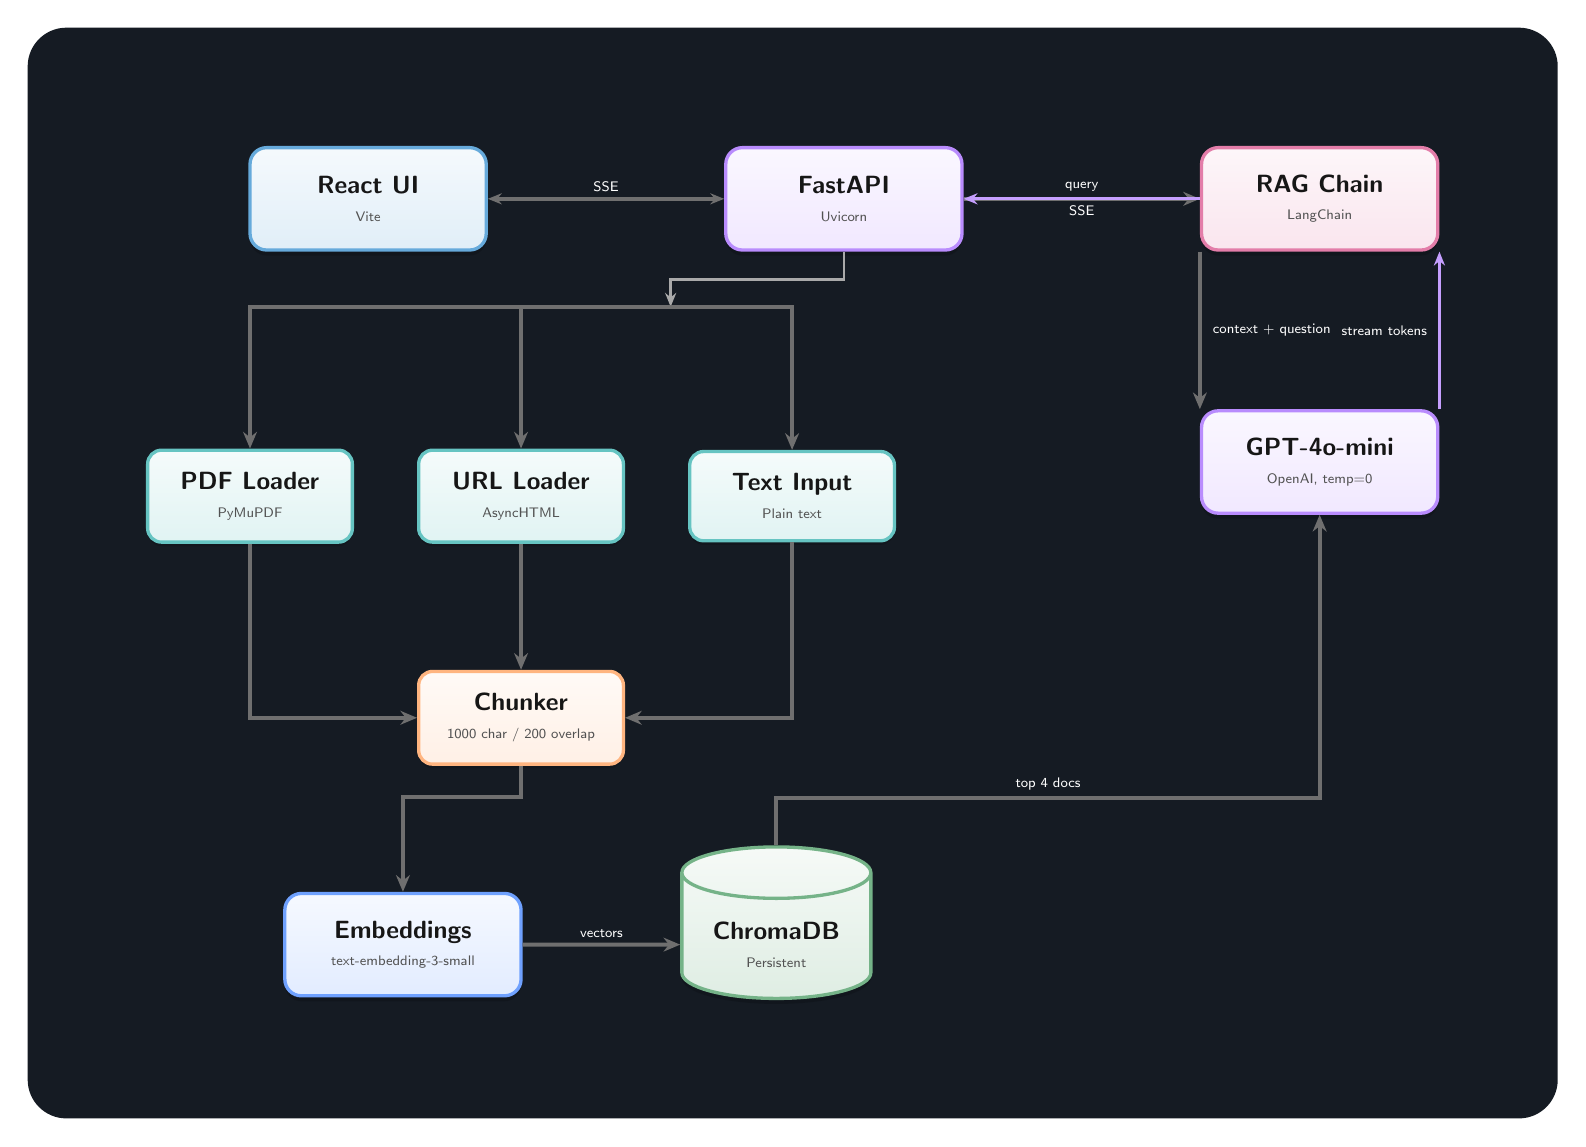
\begin{tikzpicture}

% === ROW 1: Client <-> API ===

\node[service=cyan]
  (client) {\textbf{React UI}\\[-1pt]\nsub{Vite}};

\node[service=purple, right=3cm of client]
  (api) {\textbf{FastAPI}\\[-1pt]\nsub{Uvicorn}};

\draw[flowbidi] (client) -- node[elabel, above] {SSE} (api);

% === ROW 2: Ingestion sources ===

\node[step=teal, below=2.5cm of client, xshift=-1.5cm]
  (pdf) {\textbf{PDF Loader}\\[-1pt]\nsub{PyMuPDF}};

\node[step=teal, right=0.8cm of pdf]
  (url) {\textbf{URL Loader}\\[-1pt]\nsub{AsyncHTML}};

\node[step=teal, right=0.8cm of url]
  (text) {\textbf{Text Input}\\[-1pt]\nsub{Plain text}};

% API fan-out to sources
\coordinate (fanout) at ($(api.south) + (-2.2,-0.7)$);
\draw[flowlight] (api.south) -- ++(0,-0.35) -| (fanout);
\draw[flow] (fanout) -| (pdf.north);
\draw[flow] (fanout) -| (url.north);
\draw[flow] (fanout) -| (text.north);

% === ROW 3: Chunking ===

\node[step=orange, below=1.6cm of url]
  (chunker) {\textbf{Chunker}\\[-1pt]\nsub{1000 char / 200 overlap}};

\draw[flow] (pdf.south) |- (chunker.west);
\draw[flow] (url.south) -- (chunker.north);
\draw[flow] (text.south) |- (chunker.east);

% === ROW 4: Embeddings + Vector Store ===

\node[service=primary, below=1.6cm of chunker, xshift=-1.5cm]
  (embeddings) {\textbf{Embeddings}\\[-1pt]\nsub{text-embedding-3-small}};

\node[stor=green, right=2cm of embeddings]
  (chroma) {\textbf{ChromaDB}\\[-1pt]\nsub{Persistent}};

\draw[flow] (chunker.south) -- ++(0,-0.4) -| (embeddings.north);
\draw[flow] (embeddings) -- node[elabel, above] {vectors} (chroma);

% === RIGHT COLUMN: Query Pipeline ===

\node[service=magenta, right=3cm of api]
  (rag) {\textbf{RAG Chain}\\[-1pt]\nsub{LangChain}};

\node[service=purple, below=2cm of rag]
  (llm) {\textbf{GPT-4o-mini}\\[-1pt]\nsub{OpenAI, temp=0}};

% API -> RAG
\draw[flow] (api) -- node[elabel, above] {query} (rag);

% ChromaDB -> RAG (retrieval)
\draw[flow] (chroma.north) -- ++(0,0.6) -| node[elabel, above, pos=0.25] {top 4 docs} (llm.south);

% RAG -> LLM
\draw[flow] (rag.south west) -- node[elabel, right, xshift=2pt] {context + question} (llm.north west);

% LLM -> API (streaming response)
\draw[flowlight, draw=purple!50] (llm.north east) -- node[elabel, left, xshift=-2pt] {stream tokens} (rag.south east);
\draw[flowlight, draw=purple!50] (rag.west) -- node[elabel, below] {SSE} (api.east);

% === Container: Ingestion ===
\begin{pgfonlayer}{background}
  \node[container, fit=(pdf)(url)(text)(chunker), label={[clabel]north west:INGESTION}] {};
\end{pgfonlayer}

% === Container: Storage ===
\begin{pgfonlayer}{background}
  \node[container, fit=(embeddings)(chroma), label={[clabel]north west:VECTOR STORAGE}] {};
\end{pgfonlayer}

% === Container: Query ===
\begin{pgfonlayer}{background}
  \node[container, fit=(rag)(llm), label={[clabel]north west:QUERY PIPELINE}] {};
\end{pgfonlayer}

% === Full diagram background ===
\begin{pgfonlayer}{background}
  \fill[bg, rounded corners=14pt]
    ($(current bounding box.south west) + (-1,-1)$)
    rectangle
    ($(current bounding box.north east) + (1,1)$);
\end{pgfonlayer}

\end{tikzpicture}
\end{document}
